\documentclass[xcolor=dvipsnames]{beamer} 


\usepackage[T1]{fontenc}
\usepackage[utf8]{inputenc} %caractères spéciaux
\usepackage[french]{babel} %français
\usepackage{graphicx}
\usepackage[absolute]{textpos}

\usepackage{amsmath}
\usepackage{amsfonts}
\usepackage{amssymb}

\usepackage{xspace} %symboles extensifs

\setbeamercovered{dynamic} %prevent losing position when using dynamic

\usetheme{Darmstadt}
\usecolortheme{seahorse}


\newcommand{\p}[2]{\ensuremath{\frac{\partial {#1}}{\partial {#2}}}}
\newcommand{\tot}[2]{\ensuremath{\frac{d {#1}}{d {#2}}}}

\newcommand{\vs}{\ensuremath{\mathbf{v}^s}}

\newcommand{\bfr}{\ensuremath{\mathbf{r}}}

\newcommand{\om}[1]{\ensuremath{ \mathcal{O} \left( {#1} \right) }}

\newcommand{\ttt}[1]{ \texttt{#1} }

\newcommand{\hphi}{\ensuremath{\hat{\phi}}}
\newcommand{\z}{\ensuremath{\zeta}}
\newcommand{\x}{\ensuremath{\xi}}
\newcommand{\zperp}{\ensuremath{\zeta^\perp}}
\newcommand{\lam}{\ensuremath{\lambda}}

\title[Ségrégation dans les écoulements granulaires.]{Ségrégation  dans les écoulements granulaires à surface libre.}
\date{Stage du 22 avril au 22 juillet 2013 au \\ 
\huge{Centre de dynamique non linéaire} \\ 
\small{Université de Manchester}}
\author{Nicolas Macé\\ 
\textbf{Responsable de stage :} Nico Gray}

\begin{document}

\begin{frame}
\begin{titlepage}
\end{titlepage}
\end{frame}


\section{Présentation génér	ale}
\subsection{Les milieux granulaires}
\begin{frame}

\begin{columns}[t]

  \begin{column}{5cm}
\begin{figure}[htp]
\centering
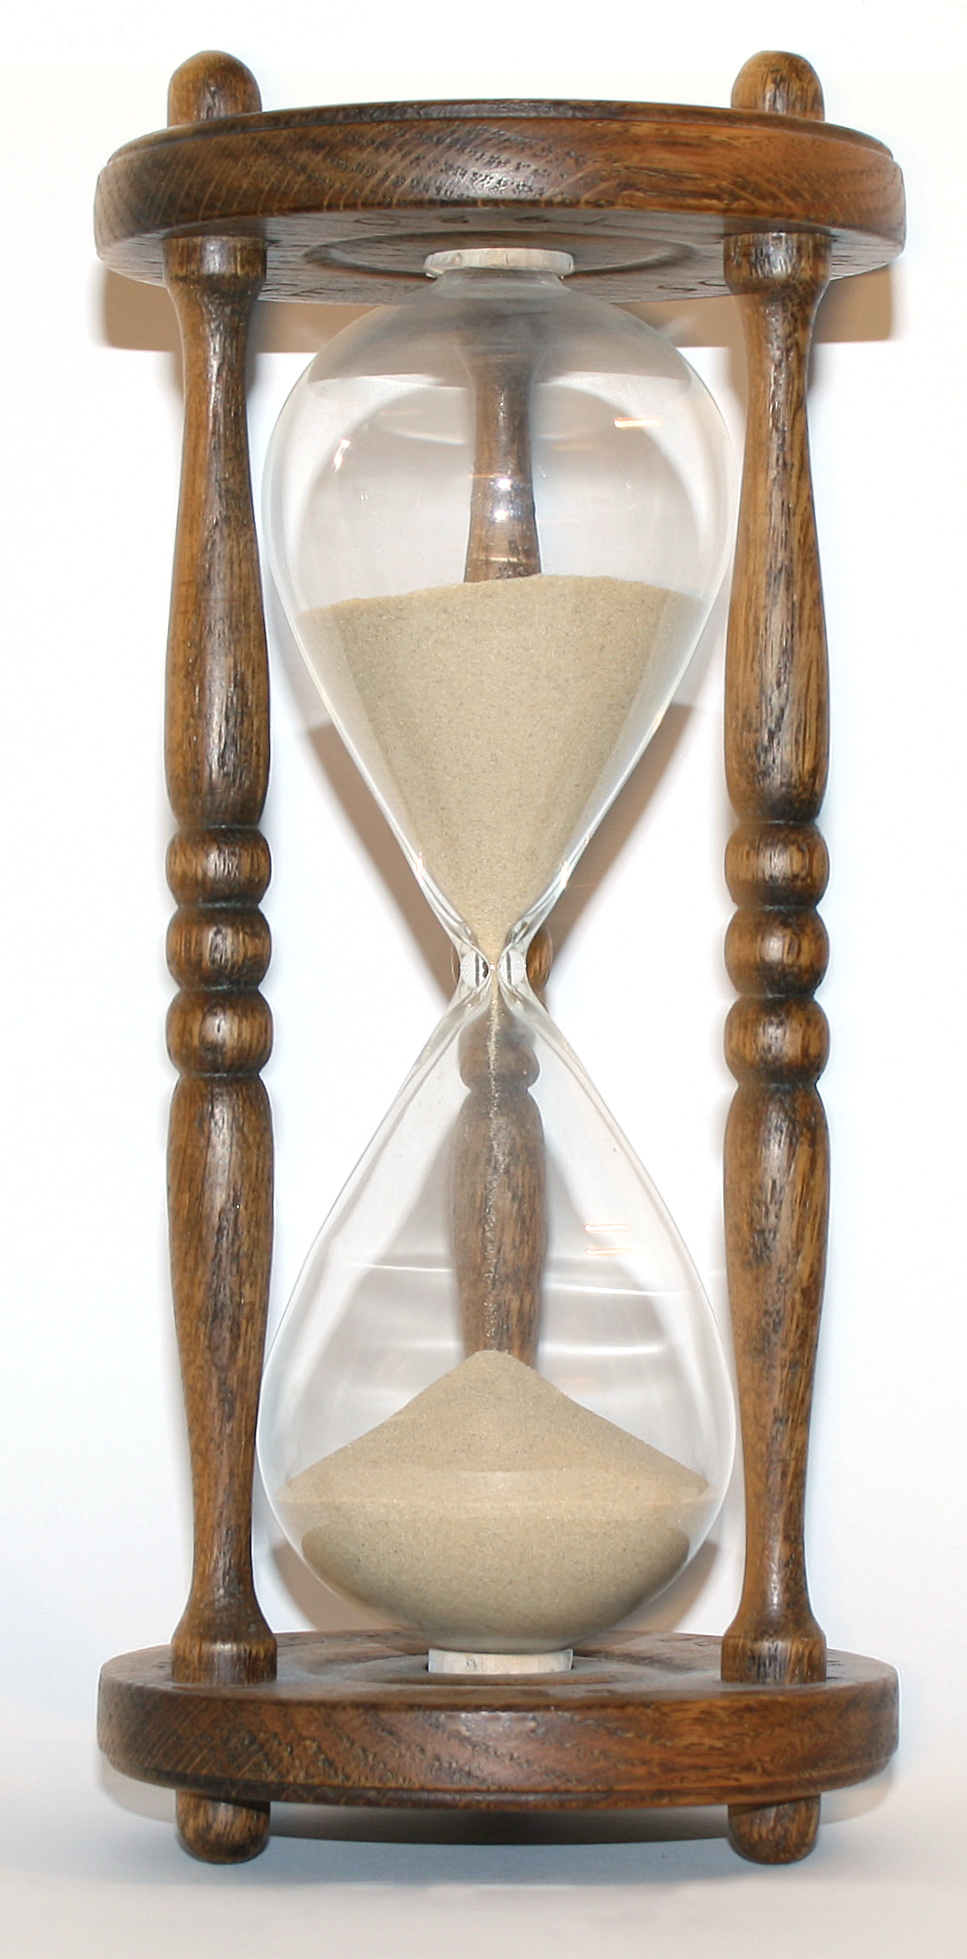
\includegraphics[scale=0.08]{img/hourglass.jpg}
\label{}
\end{figure}
  \end{column}
  
  \begin{column}{5cm}
 
\begin{itemize}

\item nature dissipative des interactions : freinage ou blocage

\item interaction par chocs et friction uniquement : $d \gtrsim 100 \text{ } \mu$m
\end{itemize}

  \end{column}
  
 \end{columns}

\end{frame}

\subsection{Le phénomène de ségrégation}
\begin{frame}

\begin{figure}[htp]
\centering
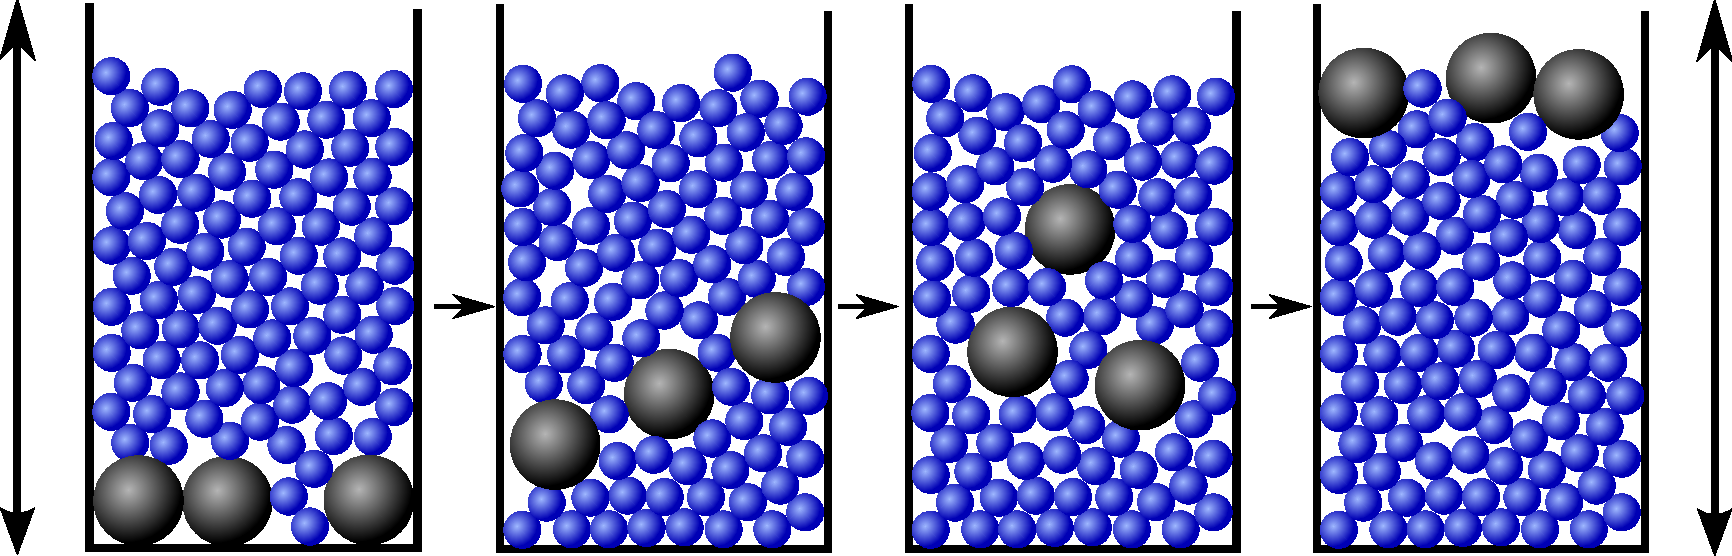
\includegraphics[scale=0.35]{img/brazil.pdf}
\label{}
\end{figure}

\begin{columns}

\begin{column}{6cm}
\[
	\p{}{t} \phi + \nabla \cdot ( \mathbf{u} \phi )  - q \p{}{z} \phi( 1 - \phi) = 0
\]
\end{column}

\begin{column}{6cm}
\[
 \text{Fraction volumique } \phi = \frac{d\tau^s}{d\tau^l + d\tau^s} 
\]
\end{column}

\end{columns}

\end{frame}

\section{Canalisation}
\subsection{Présentation}
\begin{frame}

\begin{columns}

\begin{column}{6cm}

\begin{figure}[htp]
\centering
  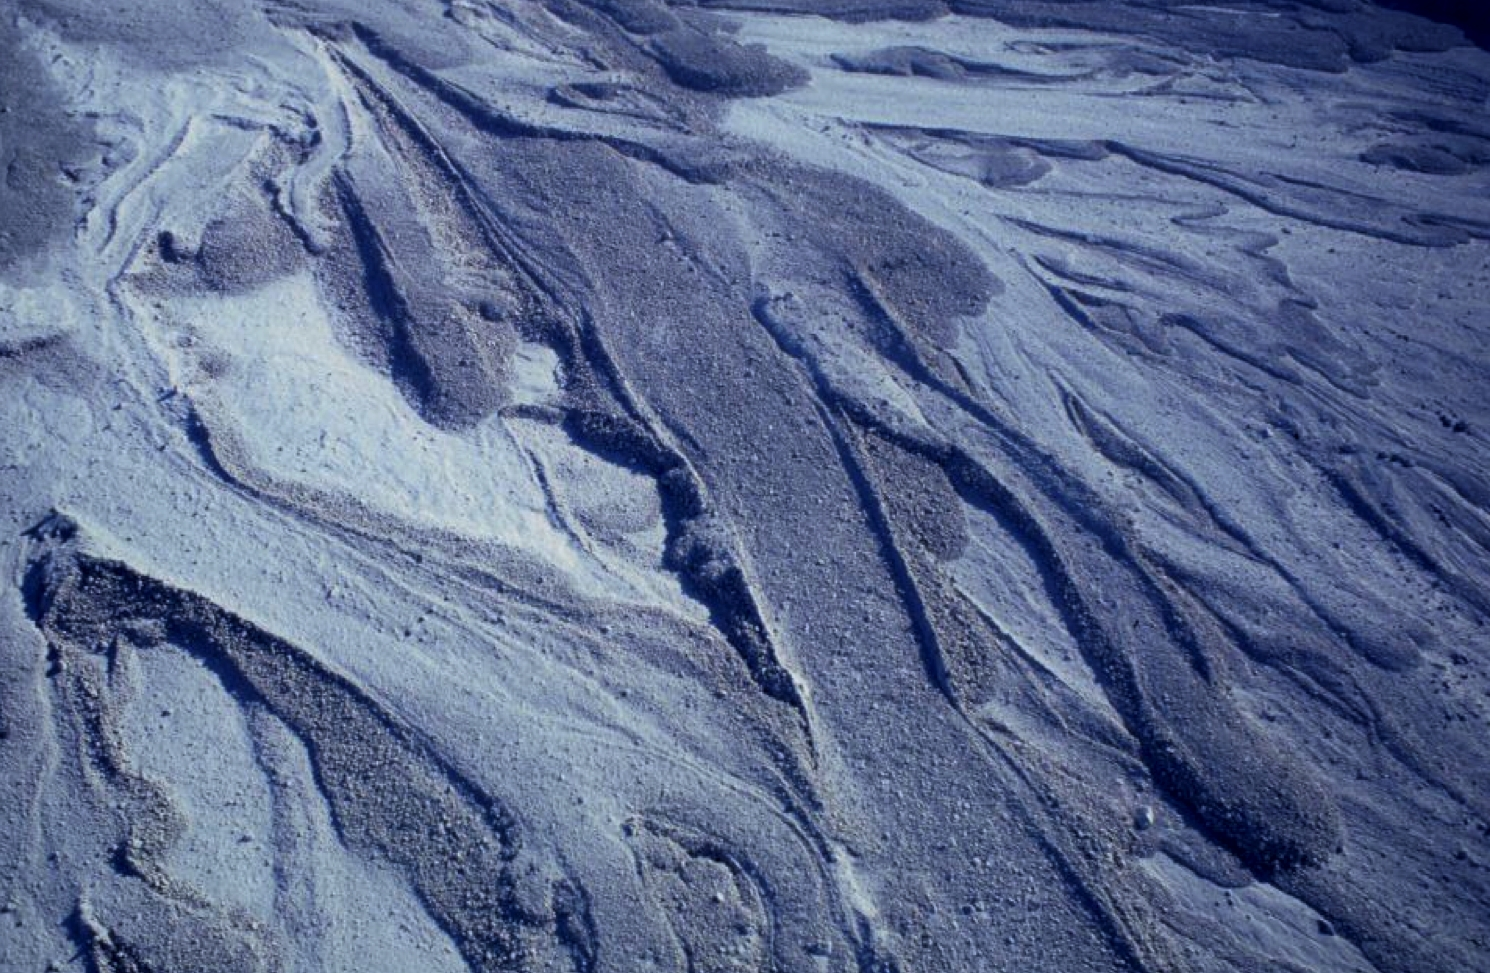
\includegraphics[width=1.\linewidth]{img/st_helen}
  \label{fig:st_helen}
\end{figure}

\end{column}

\begin{column}{6cm}

\begin{figure}
  \centering
  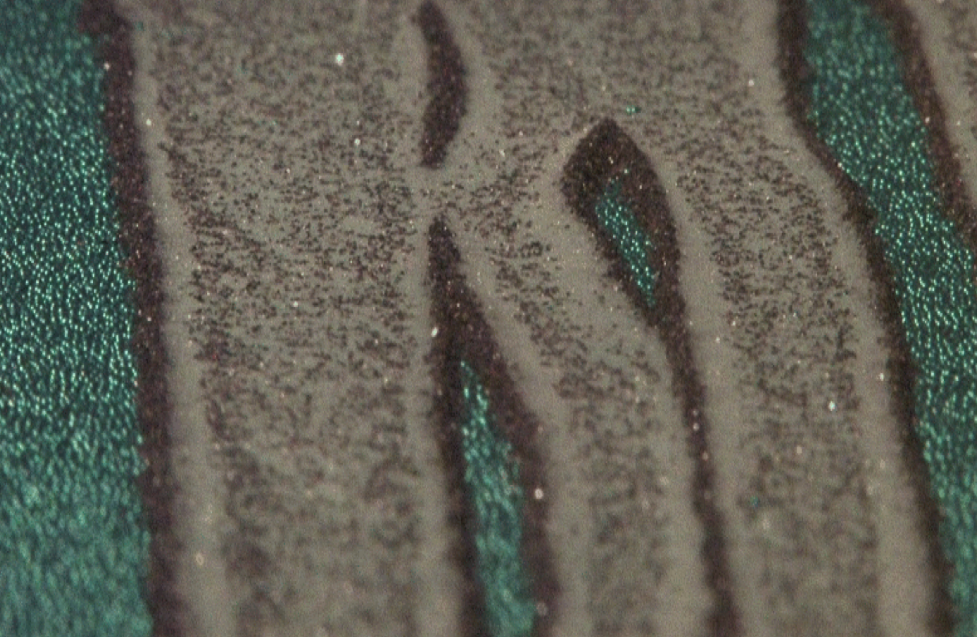
\includegraphics[width=1.\linewidth]{img/small_scale}

  \label{fig:small_scale}
\end{figure}

\end{column}

\end{columns}

~ \\
~ \\
~ \\
\begin{centering}
couplage ségrégation et convection : canalisation de l'écoulement 
\end{centering}

\begin{centering}
$\rightarrow$ analyse du phénomène \textit{pendant} l'écoulement
\end{centering}
\end{frame}

\subsection{L'expérience}
\begin{frame}

\begin{figure}[htp]
\centering
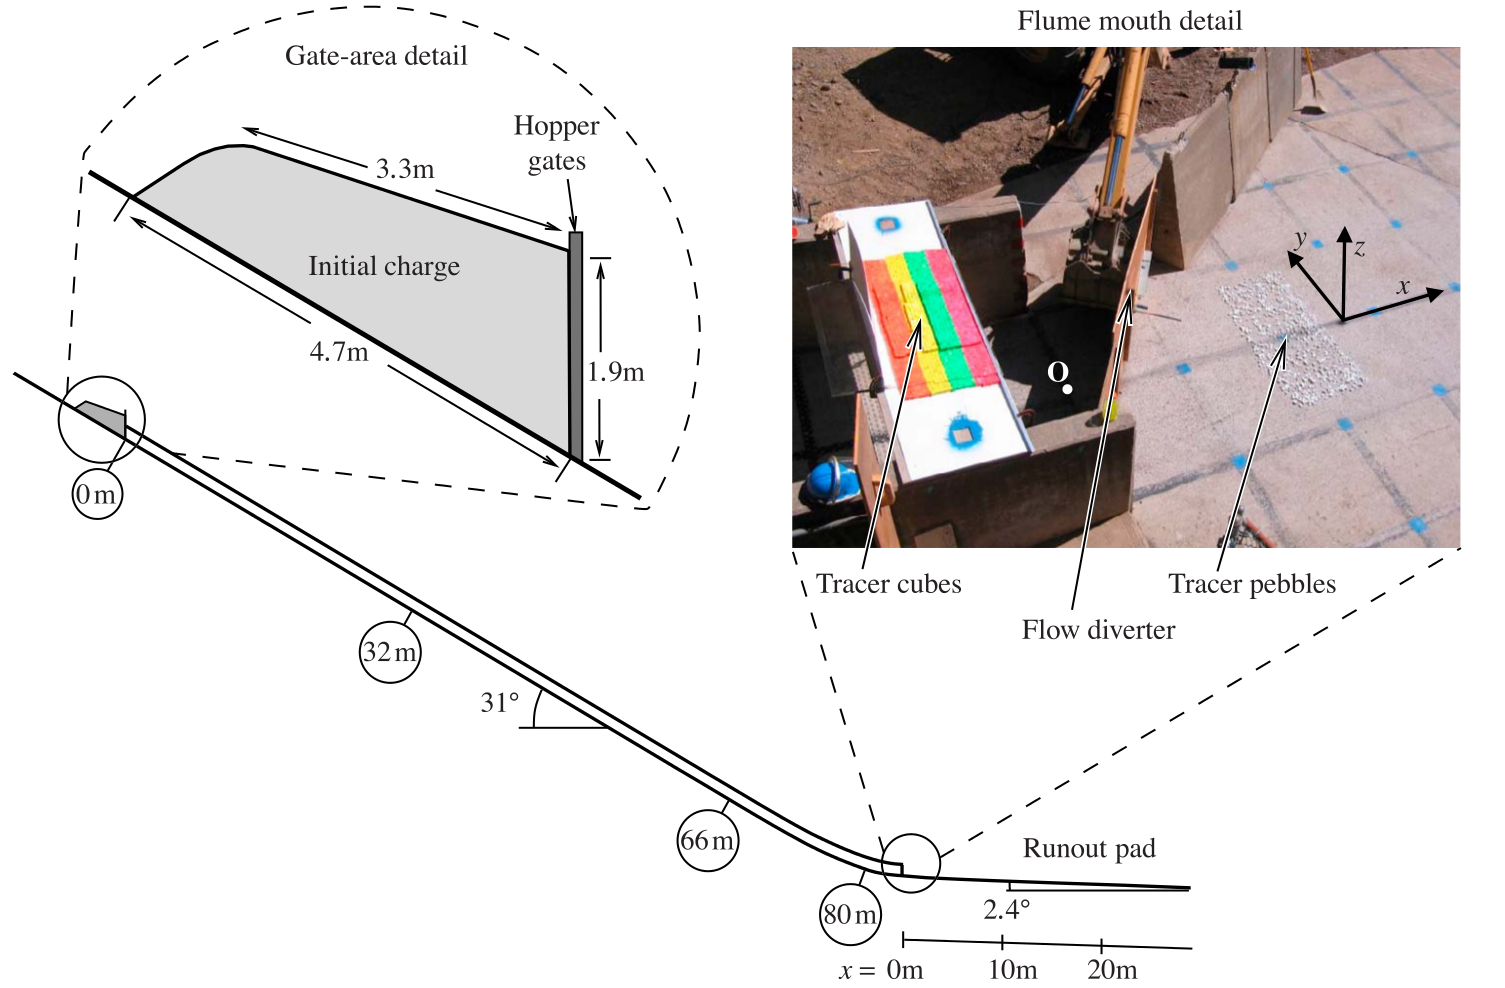
\includegraphics[scale=0.2]{img/whole_flume.png}
\label{}
\end{figure}

\end{frame}

\subsection{Modélisation}
\begin{frame}

\begin{columns}

\begin{column}{6cm}

\only<1>{
\begin{figure}[htp]
\centering
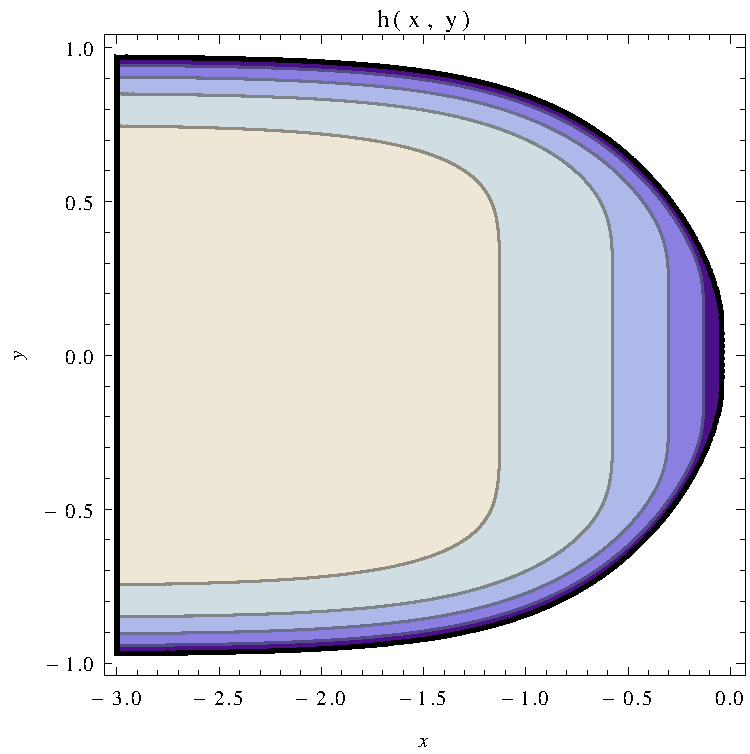
\includegraphics[scale=0.5]{img/h_contour.pdf}
\label{}
\end{figure}
}

\only<2-3>{
\begin{figure}[htp]
\centering
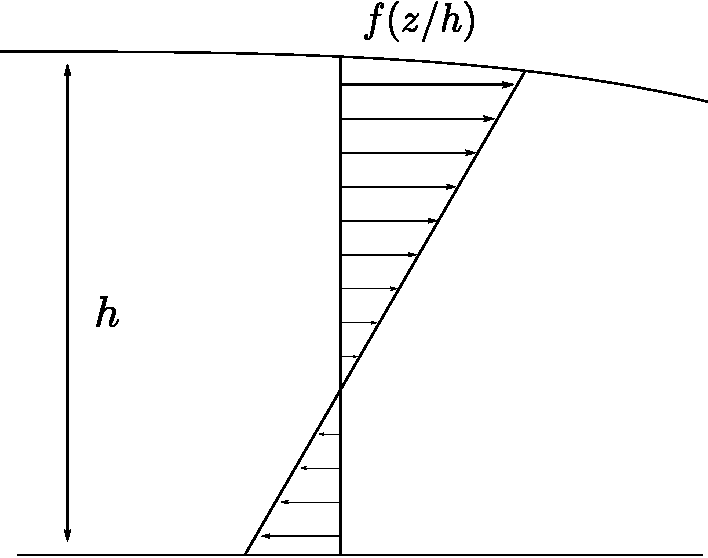
\includegraphics[scale=0.44]{img/vel_profile.pdf}
\label{}
\end{figure}
}\par

\end{column}

\begin{column}{6cm}

\only<1-2>{
\[
	h\bar{u_i}(x,y) = \int_{0}^{h} u_i(x, y, z) dz
\]

\[
	\p{}{x} h \bar u + \p{}{y} h \bar v = 0
\]

\[
	\p{z}{x_i} = \epsilon_{ij} h \bar u_j 
\]
}

\only<3>
{

\[
		\begin{pmatrix}
	u(x, y, z)\\
	v(x, y, z)\\
\end{pmatrix}
=
f \left( \frac{z}{h} \right)
\begin{pmatrix}
	\bar u(x, y) \\
	\bar v(x, y) \\
\end{pmatrix}
\]

\[
	\p{}{t} \phi + \nabla \cdot ( \mathbf{u} \phi )  - q \p{}{z} \phi( 1 - \phi) = 0
\]

}

\end{column}

\end{columns}

\end{frame}


\section{Résolution analytique}
\subsection{La méthode des caractéristiques}
\begin{frame}

Équation simplifiée :
\[
		\p{}{t} \phi - q(1 - 2 \phi) \p{}{z} \phi = 0
\]
équation aux dérivées partielles $\rightarrow$ difficile à résoudre

\[
	\frac{d \Phi}{d t} (t, z(t)) = \p{\Phi}{t} + 
	\tot{z}{t}\p{\Phi}{z} = 0
\]

\[
		\tot{z}{t}(t) = - q  \left( 1-2\Phi_0 \right)
\]
équation aux dérivées totales $\rightarrow$ simple à résoudre
\end{frame}

\begin{frame}

\begin{columns}

\begin{column}{5cm}

\begin{figure}[htp]
\centering
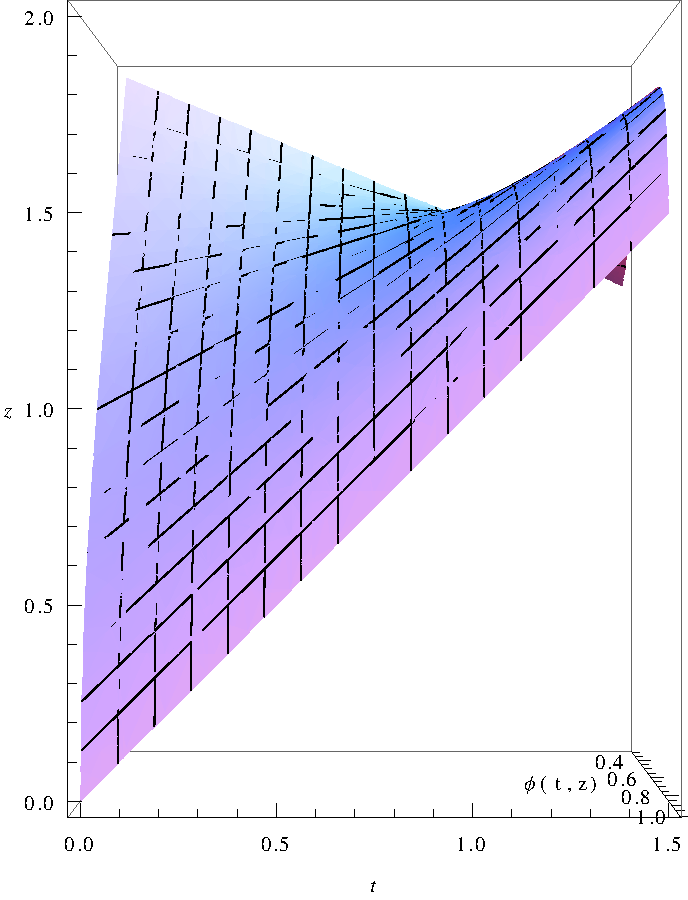
\includegraphics[scale=0.50]{img/surface.pdf}
\label{}
\end{figure}

\end{column}

\begin{column}{5cm}

\[
		\tot{z}{t}(t) = - q  \left( 1-2\Phi_0 \right)
\]

\[
\phi(0,z) = (1 - \cos z/z_0)/2
\]

\begin{itemize}
\item les caractéristiques paramétrisent la solution
\item multivaluation $\rightarrow$ onde de choc
\end{itemize}

\end{column}

\end{columns}

\end{frame}

\section{Résolution numérique}
\subsection{Le principe}
\begin{frame}

\begin{columns}

\begin{column}{6cm}

\[
		\p{}{t} \phi(t,z) + \p{}{z} f(\phi(t,z)) = 0
\]

\end{column}

\begin{column}{6cm}

\[
		\phi^{n+1}_j = \phi^n_j - \frac{\Delta t}{\Delta x} \left( F^n_{j+1/2}  - F^n_{j-1/2} \right) 
\]
\end{column}

\end{columns}

\begin{figure}[htp]
\centering
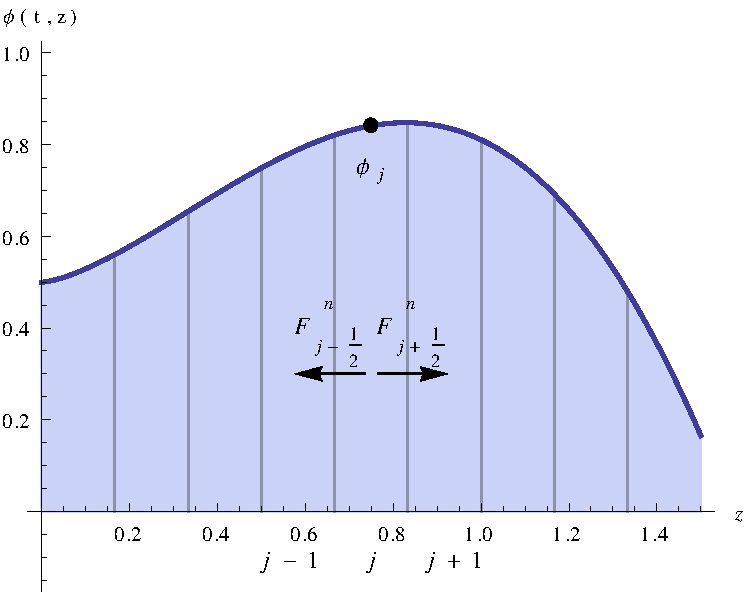
\includegraphics[scale=0.60]{img/conservative.pdf}
\label{}
\end{figure}

\end{frame}

\subsection{Quelques détails supplémentaires}
\begin{frame}

schéma numérique de Kurganov et Tadmor

\[
\begin{split}
	F^n_{j+1/2} = \frac{1}{2} \left( f(\phi^n_{j+1/2}) + f(\phi^n_{(j+1)-1/2}) \right)  \\ - \frac{1}{2} | \bar{u}^n_{j+1/2} | \left( \phi^n_{(j+1)-1/2} - \phi^n_{j+1/2} \right)
\end{split}
\]

\begin{itemize}

\item conservatif

\item précis à l'ordre 2 $\rightarrow$ faible viscosité numérique 

\item non oscillant

\item généralisable en dimension quelconque

\end{itemize}

\end{frame}


\section{Résultats}
\subsection{Plan central}
\begin{frame}

\begin{figure}[htp]
\centering
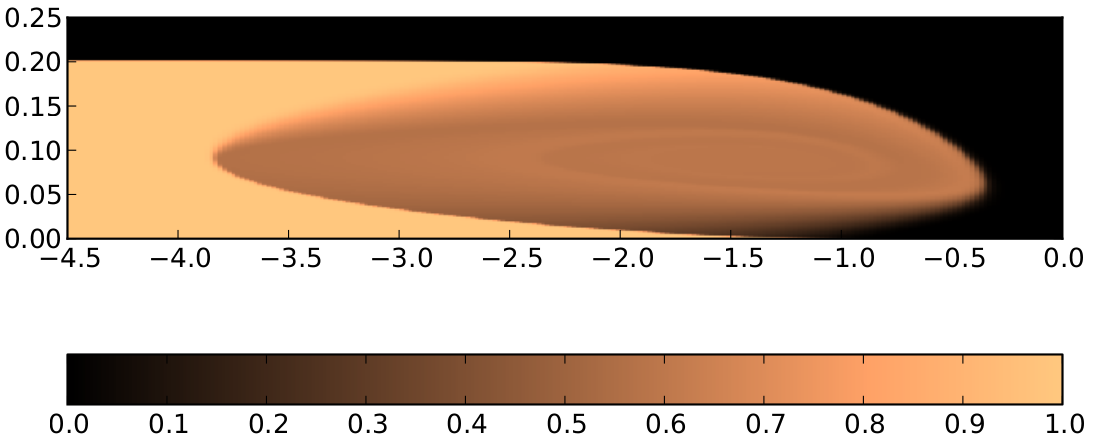
\includegraphics[scale=0.60]{img/spiral.png}
\label{}
\end{figure}

\begin{itemize}
\item structure bien connue : chocs et ondes de raréfaction
\item nouveauté : 2D compressibilité  $\rightarrow$  structure en spirale 
\end{itemize}

\end{frame}

\subsection{Écoulement complet}
\begin{frame}

\begin{figure}[htp]
\centering
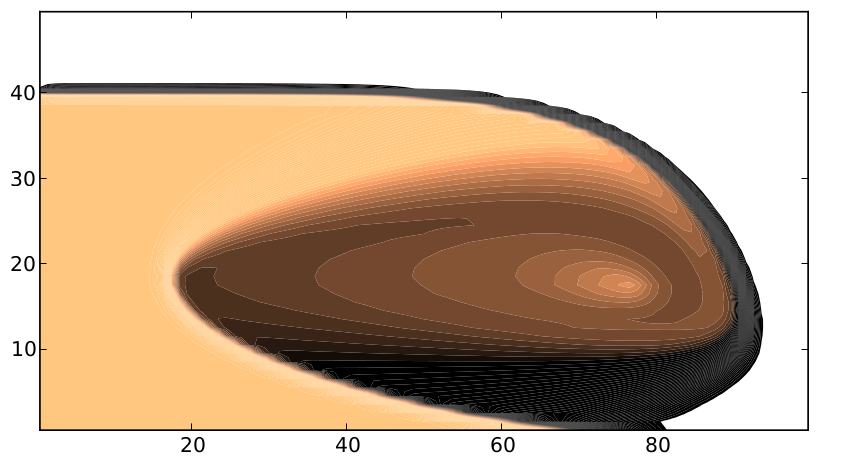
\includegraphics[scale=0.30]{img/centre.png}
\label{}
\end{figure}

\begin{columns}

\begin{column}{6cm}
\begin{figure}[htp]
\centering
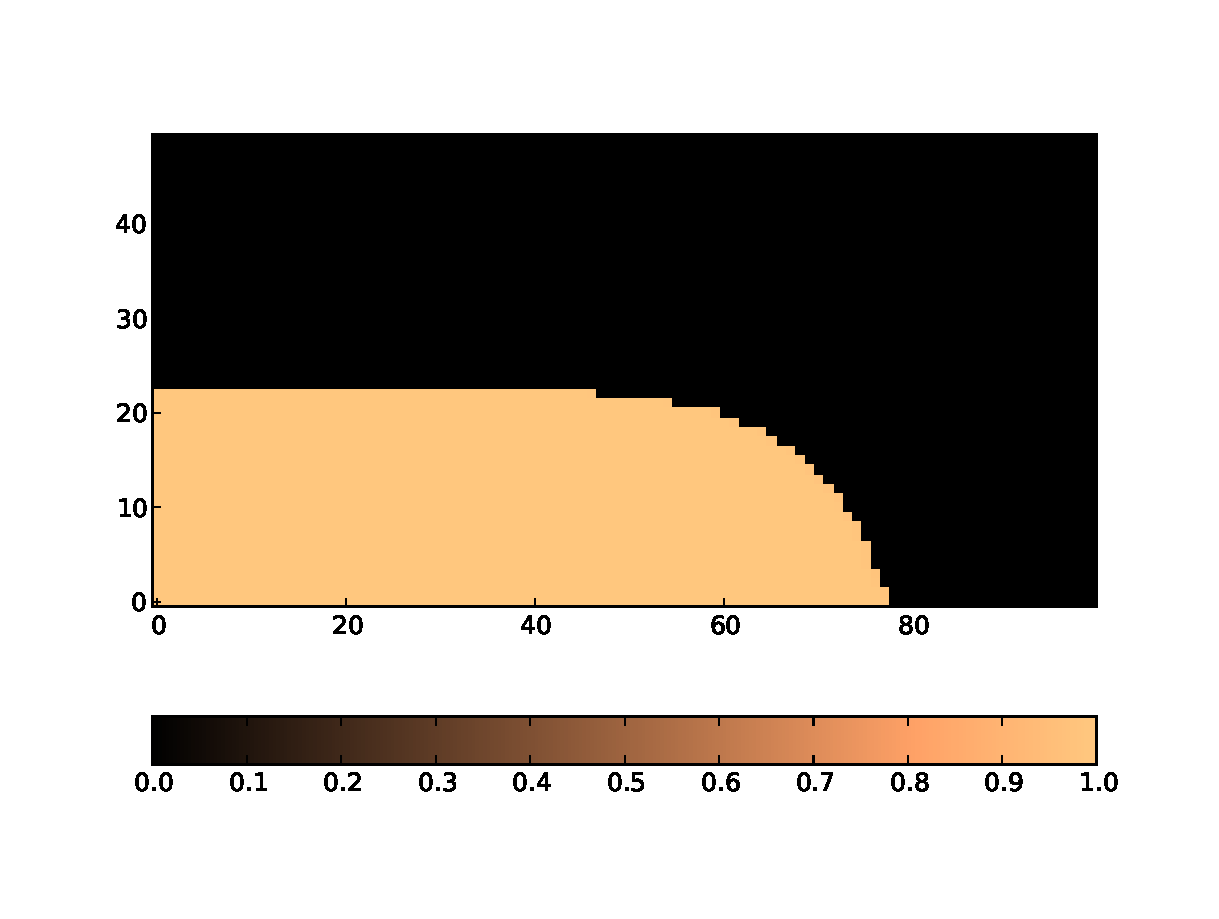
\includegraphics[scale=0.25]{img/3Dedge0.pdf}
\label{}
\end{figure}
\end{column}

\begin{column}{6cm}
\begin{figure}[htp]
\centering
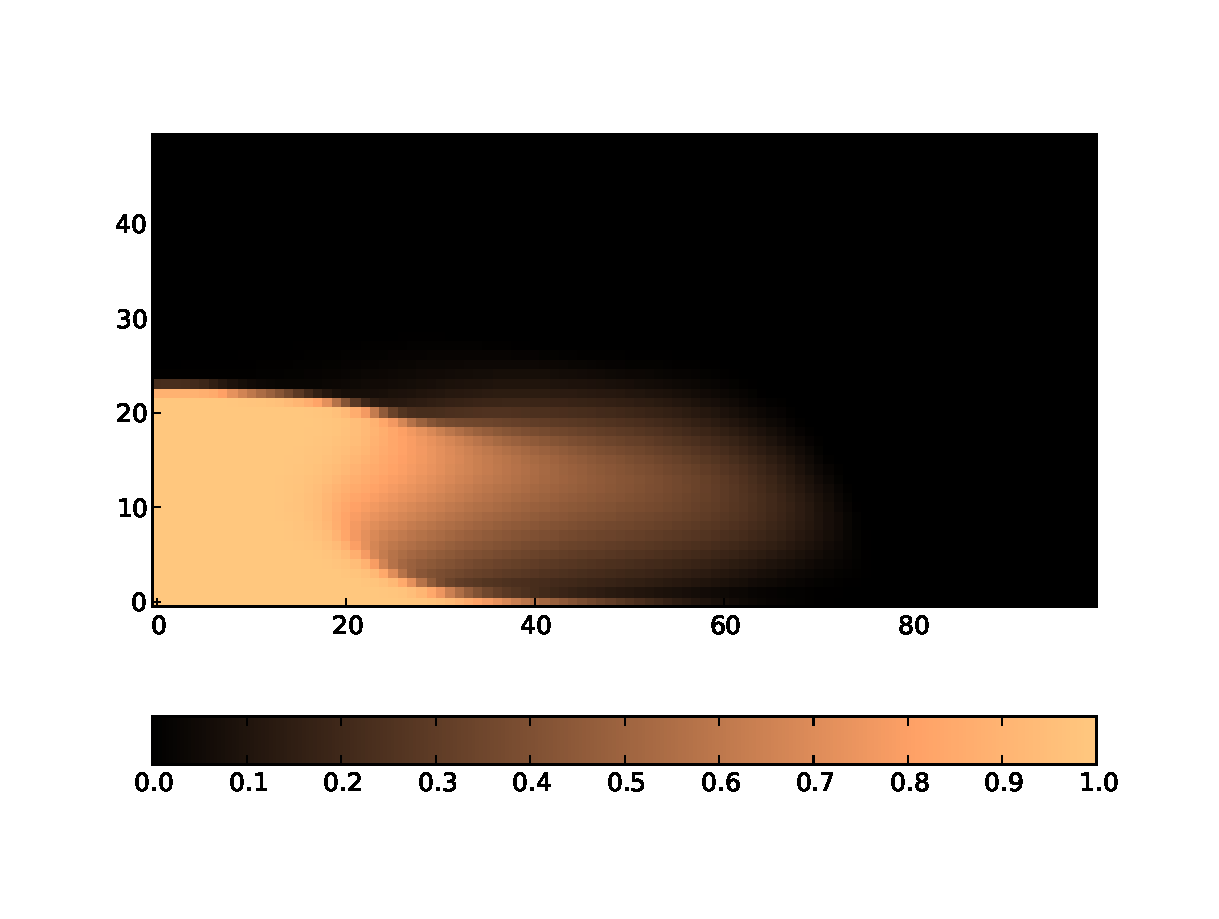
\includegraphics[scale=0.25]{img/3Dedge1.pdf}
\label{}
\end{figure}
\end{column}

\end{columns}

\end{frame}

\section{Conclusion}
\begin{frame}

\begin{itemize}
\item modélisation d'un phénomène mal compris : la ségrégation
\item relations entre physique, mathématiques et analyse numérique 
\item un domaine de la physique nouveau et en plein essor
\end{itemize}

\end{frame}

\end{document}